\documentclass[11pt,a4paper]{article}
\usepackage[utf8]{inputenc}
\usepackage{amsmath}
\usepackage{amsfonts}
\usepackage{amssymb}
\usepackage{algorithm}
\usepackage{listings}
\usepackage[pdftex]{graphicx}
\author{Anders Kaestner}
\title{MuhRec API documentation}
\date{\today}
\begin{document}
\maketitle
\section{Introduction}
\subsection{Architecture}
The reconstruction process in MuhRec is controlled by a processing engine that loads projections data, configures the processing and back projection. Projections are loaded and processed in chunks. This makes it possible to reconstruct several slices at the same time and thus save time. The chunks con be stored to disk or be used for inspection directly 
MuhRec is based on a modular concept that allows the user to dynamically add new modules in the processing chain. The processing chain is composed of two parts; a chain of preprocessing modules and a back projection module. The preprocessing chain works with a stack of projections representing a set of full sinograms. Each processing module forwards the processed data to the next module in the chain. The data from the preprocessing chain is forwarded to the back projection module after completed processing. 


\subsection{Library structure}
\begin{figure}
\centering
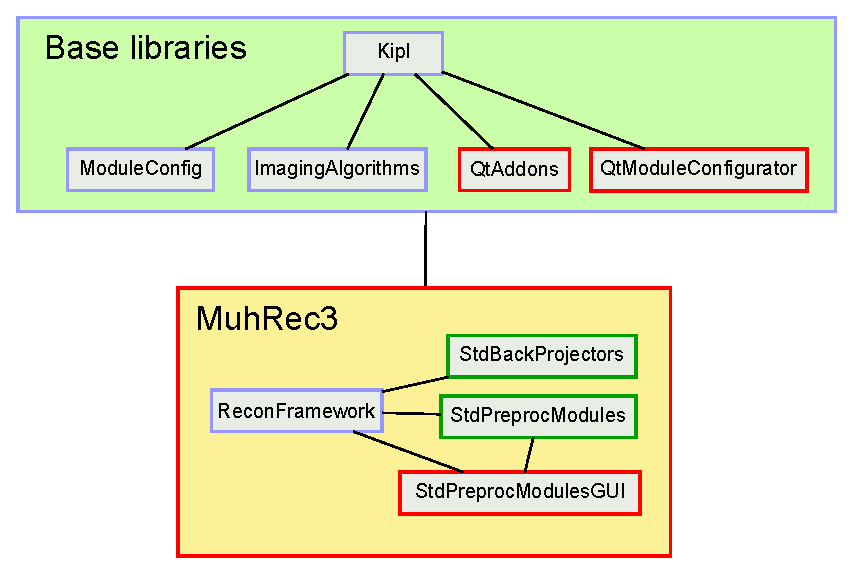
\includegraphics[width=0.75\textwidth]{figures/KiplComponents.pdf}
\caption{Library dependencies for MuhRec. Libraries framed in red are GUI components.}
\end{figure}
\section{The image class}
\section{Preprocessing modules}
\section{Back projection modules}
Back projection modules are constructed in a similar way as the preprocessing modules. A back projector library consists of a set of interface functions to create and destroy instances of the implemented back projection modules. There shall also be a function that provides a list of available modules and their specific configuration parameters. This interface is implemented as the four functions
 GetModuleList, GetModule, Destroy, and LibVersion.

\lstset{language=C++ %,
%                basicstyle=\ttfamily,
%                keywordstyle=\color{blue}\ttfamily,
%                stringstyle=% \color{red}\ttfamily,
%                commentstyle=\color{green}\ttfamily,
%                morecomment=[l][\color{magenta}]{\#}
}

In the case of GUI operation the function GetModuleList is called the obtain a list of modules provided by the shared object file. The function takes one input string that is used to identify if the caller can handle the modules provided by the library. In the case of back projector modules the caller shall probe with the string "muhrecbp" without capitalization. The function then fills the STL map<string, map<string,string>> instance provided by the caller with module names and lists of parameters associated with each module. The listing below show the GetModuleList function from the StdBackProj library. The module name used as key in the map will later be used in the GetModule call to identify the module to create.
\begin{lstlisting}
DLL_EXPORT int GetModuleList(const char * application, void *listptr)
{
  using namespace std; // This is only for formatting 
                                      // normally otherwise use std::
  if (strcmp(application,"muhrecbp"))
    return -1;

  map<string, map<string, string> > *pmodulelist =
    reinterpret_cast<map<string, map<string, string> > *>(listptr);

  map<string, map<string, string> > & modulelist = *pmodulelist;

  MultiProjectionBP mpbp;
  modulelist["MultiProjBP"] = mpbp.GetParameters();

  MultiProjectionBPparallel mpbpp; 
  modulelist["MultiProjBPparallel"]=mpbpp.GetParameters();

  NearestNeighborBP nnbp;
  modulelist["NearestNeighborBP"]=nnbp.GetParameters();

	return 0;
}
\end{lstlisting}

Modules are provided using a factory function that creates instances of the module specified by the argument \emph{name}. Like all other interface functions this also requires the identification through the string \emph{application}. The function takes a third argument that is a reference to an allocated interactor instance. The role of the interactor is to provide a means to communicate and control between the application and the module. The factory 

\begin{lstlisting}
DLL_EXPORT void * GetModule(const char *application, 
                            const char * name, 
                            void *vinteractor)
{
  if (strcmp(application,"muhrecbp"))
    return NULL;

  InteractionBase *interactor = 
    reinterpret_cast<InteractionBase *>(vinteractor);
  
  if (name!=NULL) {
    std::string sName=name;

    if (sName=="MultiProjBP")
      return new MultiProjectionBP(interactor);

    if (sName=="MultiProjBPparallel")
      return new MultiProjectionBPparallel(interactor);

    if (sName=="NearestNeighborBP")
      return new NearestNeighborBP(interactor);
		
    if (sName=="MultiProjBPparallel")
      return new MultiProjectionBPparallel(interactor);
  }

  return NULL;
}
\end{lstlisting}

It is good style to provide a destroyer function as part of the library interface. The use of a destroyer guarantees a clear deallocation of the created instances. The destroyer takes two arguments; \emph{application} that is shall be a string containing the name of the application in the case of back projection modules this is muhrecbp. This string prevents the function from deleting the wrong type of data. The second argument is a pointer to the object to delete. 
\begin{lstlisting}
DLL_EXPORT int Destroy(const char *application,void *obj)
{
  kipl::logging::Logger logger("StdBackProj::Destroy");
  
  if (strcmp(application,"muhrecbp"))
    return -1;

  std::ostringstream msg;
  if (obj!=NULL) {
    BackProjectorBase *module=reinterpret_cast<BackProjectorBase *>(obj);
    delete module;
  }
  
  return 0;
}
\end{lstlisting}

\begin{lstlisting}
DLL_EXPORT int LibVersion()
{
	return -1;
}
\end{lstlisting}

\begin{algorithm}
\begin{lstlisting}
#include "stdafx.h"
#include "../include/StdBackProjectors.h"
#include <BackProjectorBase.h>
#include <InteractionBase.h>
#include "../include/MultiProjBP.h"
#include "../include/MultiProjBPparallel.h"
#include "../include/NNMultiProjBP.h"

#include <cstdlib>
#include <string>

DLL_EXPORT void * GetModule(const char *application, 
                                                    const char * name, 
                                                    void *vinteractor)
{
    if (strcmp(application,"muhrecbp"))
		return NULL;

	InteractionBase *interactor=reinterpret_cast<InteractionBase *>(vinteractor);
	if (name!=NULL) {
		std::string sName=name;

		if (sName=="MultiProjBP")
			return new MultiProjectionBP(interactor);

		if (sName=="MultiProjBPparallel")
			return new MultiProjectionBPparallel(interactor);

		if (sName=="NearestNeighborBP")
			return new NearestNeighborBP(interactor);
		if (sName=="MultiProjBPparallel")
			return new MultiProjectionBPparallel(interactor);

	}

	return NULL;
}

DLL_EXPORT int Destroy(const char *application,void *obj)
{
	kipl::logging::Logger logger("StdBackProj::Destroy");
    if (strcmp(application,"muhrecbp"))
		return -1;

	std::ostringstream msg;
	if (obj!=NULL) {
		BackProjectorBase *module=reinterpret_cast<BackProjectorBase *>(obj);
		delete module;
	}

	return 0;
}

DLL_EXPORT int LibVersion()
{
	return -1;
}

DLL_EXPORT int GetModuleList(const char * application, void *listptr)
{
    if (strcmp(application,"muhrecbp"))
		return -1;

	std::map<std::string, std::map<std::string, std::string> > *modulelist=reinterpret_cast<std::map<std::string, std::map<std::string, std::string> > *>(listptr);

	MultiProjectionBP mpbp;
	modulelist->operator []("MultiProjBP")=mpbp.GetParameters();

	MultiProjectionBPparallel mpbpp;
	modulelist->operator []("MultiProjBPparallel")=mpbpp.GetParameters();

	NearestNeighborBP nnbp;
	modulelist->operator []("NearestNeighborBP")=nnbp.GetParameters();

	return 0;
}

\end{lstlisting}
\caption{Test}
\end{algorithm}
\end{document}